As introduced in section \ref{SEC:L2PAIRWISE}, the use of the metric $\mathbb{L}^2$
for the pairwise alignment of functions leads to a series of issues, which make
its use unsuitable for this problem. This is why we will use differential
geometry techniques to find a suitable metric. In particular, given two
functions $f_1$, $f_2$ and $\gamma \in \Gamma$, we will look for a metric that
remains invariant to warpings in the domain, i. e.,
$d(f_1, f_2) = d(f_1 \circ \gamma, f_2 \circ \gamma)$.

For this purpose we will use the Fisher-Rao metric. This riemannian metric was
introduced in 1945 by C. R. Fisher [Ref to fisher paper] in a version on the
space of probability distributions. In our case we will use a non-parametric
version, slightly different from the original one, defined on the space of
signed measures. This metric plays a very important role in information
geometry, and it is the only metric that possesses this property of
invariance \cite{Cencov1982}.

A riemannian metric is an application that assigns an inner product at each
point of variety on its tangent space that varies smoothly from point to point.
This will give us local notions of angles, length of curves or volumes.

In our case our manifold will be formed by the set of absolutely continuous
functions $\mathcal{F}$, that is, those functions whose derivative exists a.e.
and belongs to $\mathbb{L}^2$. We will endow $\mathcal{F}$ with the
Fisher-Rao metric.

Let $f \in \mathcal{F}$  and $v_{1}, v_{2} \in T_{f}(\mathcal{F})$,
the Fisher-Rao metric is defined as

\begin{equation}[EQ:FRAO]{Fisher-Rao metric}
\left\langle\left\langle v_{1}, v_{2}\right\rangle\right\rangle_{f}=
\frac{1}{4} \int_{0}^{1} \dot{v}_{1}(t) \dot{v}_{2}(t) \frac{1}{|\dot{f}(t)|}dt,
\end{equation}
where $\dot v$ denotes the derivative.

Using this local notion of inner product, we will be able to calculate the
length of a differentiable path in our manifold
$\alpha(\tau) \subset \mathcal{F}$ integrating through it, i.e.,

\begin{equation}[]{Length of path}
L[\alpha] = \int_0^1 \langle \langle \dot \alpha(\tau), \dot \alpha(\tau)
\rangle \rangle_{\alpha(\tau)} d\tau.
\end{equation}

This will allow us to define the distance between two points of the
manifold $f_1, f_2 \in \mathcal{F}$ as the length of the geodesic path, or shortest
path, which connects $f_1$ and $f_2$,

\begin{equation}[]{Length of shortest path}
d_{F R}\left(f_{1}, f_{2}\right)=\inf _{\alpha :[0,1]
\rightarrow \mathcal{F}, \alpha(0)=f_{1}, \alpha(1)=f_{2}} L[\alpha] \, .
\end{equation}

Finding the geodesic path directly is computationally unapproachable,
for this reason we will introduce the \textbf{square root slope function} (SRSF)
transform, which will greatly simplify this computation.

\begin{figure}[Geodesic path in $\mathcal{F}$]{FIG:GEODESIC}{Geodesic path in $\mathcal{F}$ and the corresponding SRSF's}
  \subfigure[SBFIG:GEODESIC1]{Some steps of the geodesic path between $f_1$ and $f_2$}{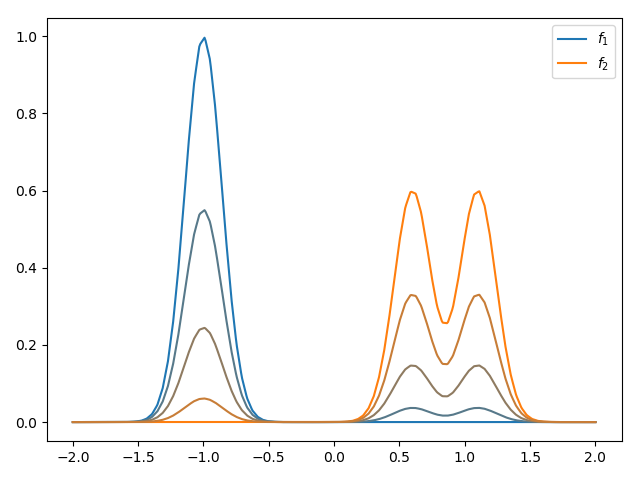
\includegraphics[width=7.5cm]{geodesic}} \quad
  \subfigure[SBFIG:GEODESIC2]{SRSF of the path}{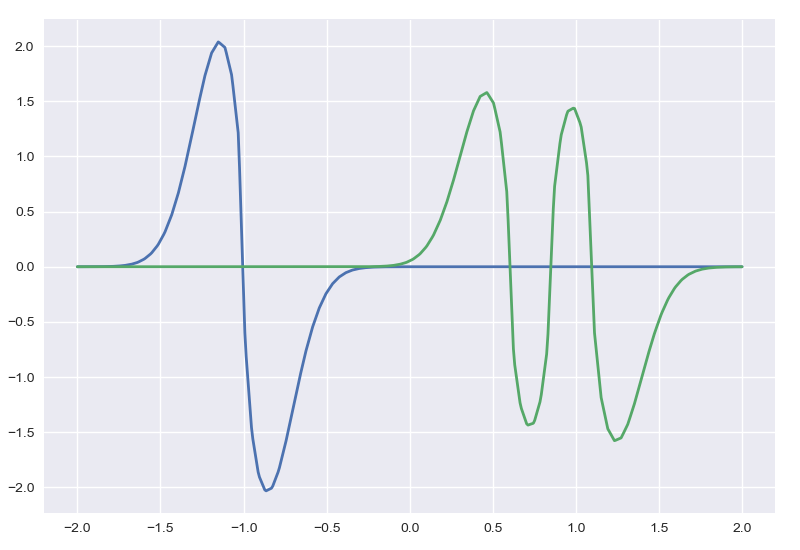
\includegraphics[width=7.5cm]{srsf-geodesic}}
\end{figure}

Given $f \in \mathcal{F}$, its SRSF is defined as
$SRSF\{f\} = \operatorname{sgn}{(\dot f)} \sqrt{\dot f}$. To simplify notation, in the
subsequent sections, we will denote the SRSF of a function
$f_i \in \mathcal{F}$ as $q_i$.

Under this transformation, the Fisher-Rao metric becomes the usual metric
in $\mathbb{L}^2$, so that the distance between two functions will be
calculated using the distance $\mathbb{L}^2$ of their corresponding
SRSF's, i.e.,  $d_{FR}(f_1, f_2) = \| q_1 - q_2 \|_{\mathbb{L}^2}$. A proof of
this result is included in appendix \ref{SEC:ACTION}.

Taking advantage of this characterization we will take our functions to the
SRSF's space to perform our analysis efficiently, and then transform the result
to the original space, because the SRSF establishes a map up to constant between
$\mathcal{F}$ and the space of SRSF's with the $\mathbb{L}^2$ metric.
A consequence is that the computation of geodesics shown in
\ref{FIG:GEODESIC} becomes in a straight line
between SRSFs,
\begin{equation}[]{Straight line of SRSFs}
\alpha(\tau) = (1 - \tau)q_1 + \tau q_2 \quad 0 \le \tau \le 1.
\end{equation}

Given $\gamma \in \Gamma$, when it is calculated the SRSF of $f \circ \gamma$,
due to the chain rule, we can observe that
$SRSF\{f \circ \gamma\} = \operatorname{sgn}(\dot{f} \circ \gamma) \sqrt{\dot f \circ \gamma}
\sqrt{\dot \gamma} = (q \circ \gamma) \sqrt{\dot \gamma}$. To simplify the
notation we  will denote the SRSF of this composition as $(q, \gamma)$.
Using this fact, we can proof that the action of $\Gamma$ on $\mathscr{F}$ is an
action by isometries, i.e, given $f  \in \mathscr{F}$ and $\gamma \in \Gamma$
the composition $f \circ \gamma$ preserves the metric.
A proof of this result is given in the appendix \ref{SEC:ACTION}.
Figure \ref{FIG:ACTIONS} shows a diagram with the action of the composition
in the different spaces.

\begin{figure}[Action of $\Gamma$]{FIG:ACTIONS}{Action of $\Gamma$}

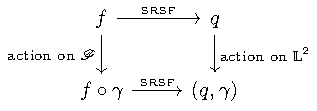
\includegraphics[width=8cm]{actions}

\end{figure}
